\documentclass[12pt, twoside]{article}
\usepackage[letterpaper, margin=1in, headsep=0.5in]{geometry}
\usepackage[english]{babel}
\usepackage[utf8]{inputenc}
\usepackage{amsmath}
\usepackage{amsfonts}
\usepackage{amssymb}
\usepackage{tikz}
\usetikzlibrary{quotes, angles}
\usepackage{graphicx}
%\usepackage{pgfplots}
%\pgfplotsset{width=10cm,compat=1.9}
%\usepgfplotslibrary{statistics}
%\usepackage{pgfplotstable}
%\usepackage{tkz-fct}
%\usepackage{venndiagram}
\usepackage{enumitem}
\usepackage{multicol}


\usepackage{fancyhdr}
\pagestyle{fancy}
\fancyhf{}
\fancyhead[LE]{\thepage}
\fancyhead[RO]{\thepage \\Name: \hspace{4cm} \,\\}
\fancyhead[LO]{BECA / Dr. Huson / Geometry 10th Grade\\* Unit 9: Congruence transformations \\ 28 February 2020}

\renewcommand{\headrulewidth}{0pt}

\begin{document}
\subsubsection*{9.5b Exam: Rigid motions including translation, reflection, rotation}
  \begin{enumerate}

  \item Slide $\triangle ABC$ to the right three and up four. Label the image $\triangle A'B'C'$.
    \begin{center}
        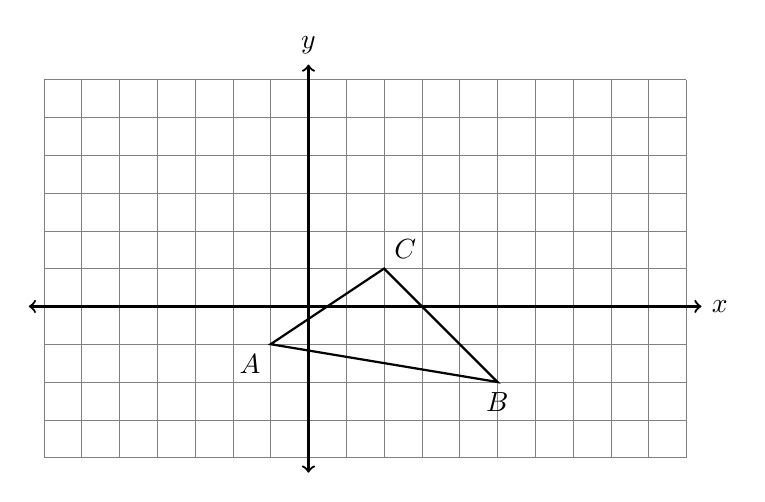
\begin{tikzpicture}[scale=.48]
        \draw [help lines] (-7,-4) grid (10,6);
        \draw [thick, <->] (-7.4,0) -- (10.4,0) node [right] {$x$};
        \draw [thick, <->] (0,-4.4)--(0,6.4) node [above] {$y$};  
        \draw [thick]
          (-1,-1) node[below left] {$A$}--
          (5,-2) node[below] {$B$}--
          (2,1) node[above right] {$C$}--cycle;  
      \end{tikzpicture}
    \end{center}

  \item Translate $\triangle DEF$ by $(x,y) \rightarrow (x+3, y-5)$. Label the image $\triangle D'E'F'$.
  \begin{center}
      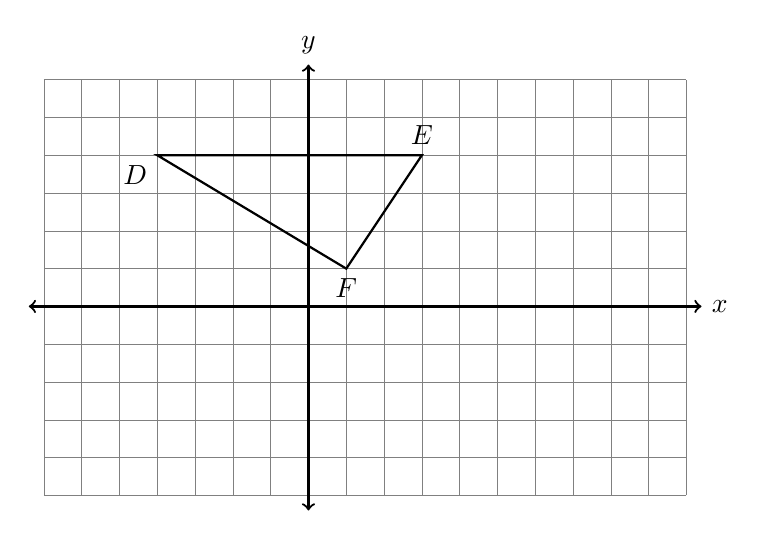
\begin{tikzpicture}[scale=.48]
      \draw [help lines] (-7,-5) grid (10,6);
      \draw [thick, <->] (-7.4,0) -- (10.4,0) node [right] {$x$};
      \draw [thick, <->] (0,-5.4)--(0,6.4) node [above] {$y$};  
      \draw [thick]
        (-4,4) node[below left] {$D$}--
        (3,4) node[above] {$E$}--
        (1,1) node[below] {$F$}--cycle;  
    \end{tikzpicture}
  \end{center}

  \begin{multicols}{2}
    [\item Which of the following would map $\triangle CAT \rightarrow \triangle C'A'T'$?]  \vspace{0.5cm}
    \begin{itemize}
      \item[T \quad F \quad] Reflected across the $y$-axis
      \item[T \quad F \quad] Translated six to the left, down zero
      \item[T \quad F \quad] Reflected across the $y$-axis, then slid to the left two
      \item[T \quad F \quad] $(x,y) \rightarrow (x-6, y+0)$
      \item[T \quad F \quad] Rotated $90^\circ$ counterclockwise around the origin
      \item[T \quad F \quad] Reflected across the line $x=-1$
    \end{itemize}
    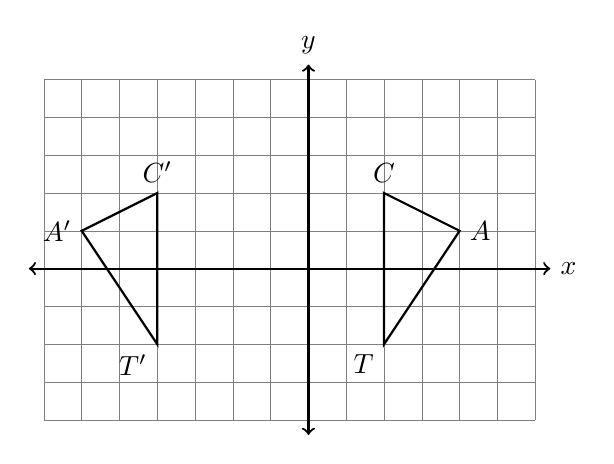
\begin{tikzpicture}[scale=.48]
      \draw [help lines] (-7,-4) grid (6,5);
      \draw [thick, <->] (-7.4,0) -- (6.4,0) node [right] {$x$};
      \draw [thick, <->] (0,-4.4)--(0,5.4) node [above] {$y$};  
      \draw [thick]
      (2,2) node[above] {$C$}--
      (4,1) node[right] {$A$}--
      (2,-2) node[below left] {$T$}--cycle;
      \draw [thick]
      (-4,2) node[above] {$C'$}--
      (-6,1) node[left] {$A'$}--
      (-4,-2) node[below left] {$T'$}--cycle;
    \end{tikzpicture}
  \end{multicols}

  \begin{multicols}{2}
    [\item Which of the following would map $\triangle CAT \rightarrow \triangle C'A'T'$?]  \vspace{0.5cm}
    \begin{itemize}
      \item[T \quad F \quad] Reflected across the $y$-axis
      \item[T \quad F \quad] Translated six to the left, down zero
      \item[T \quad F \quad] Reflected across the $y$-axis, then slid to the left two
      \item[T \quad F \quad] $(x,y) \rightarrow (x-6, y+0)$
      \item[T \quad F \quad] Rotated $90^\circ$ counterclockwise around the origin
      \item[T \quad F \quad] Reflected across the line $x=-1$
    \end{itemize}
    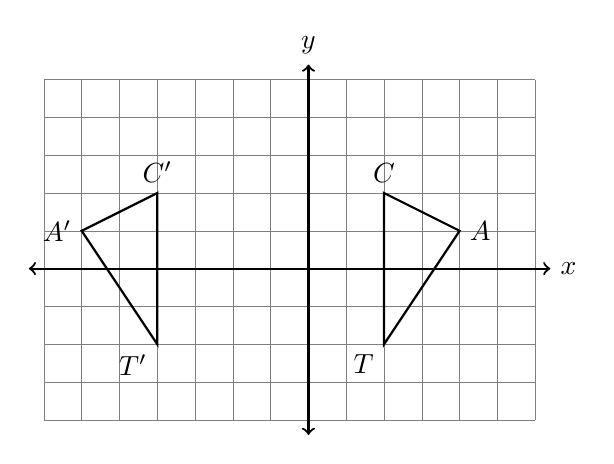
\begin{tikzpicture}[scale=.48]
      \draw [help lines] (-7,-4) grid (6,5);
      \draw [thick, <->] (-7.4,0) -- (6.4,0) node [right] {$x$};
      \draw [thick, <->] (0,-4.4)--(0,5.4) node [above] {$y$};  
      \draw [thick]
      (2,2) node[above] {$C$}--
      (4,1) node[right] {$A$}--
      (2,-2) node[below left] {$T$}--cycle;
      \draw [thick]
      (-4,2) node[above] {$C'$}--
      (-6,1) node[left] {$A'$}--
      (-4,-2) node[below left] {$T'$}--cycle;
    \end{tikzpicture}
  \end{multicols}

  \item Determine and state the transformation mapping $\triangle DEF$ onto $\triangle ABC$. Also, make a mapping table of the coordinate pairs.
    \begin{flushright}
        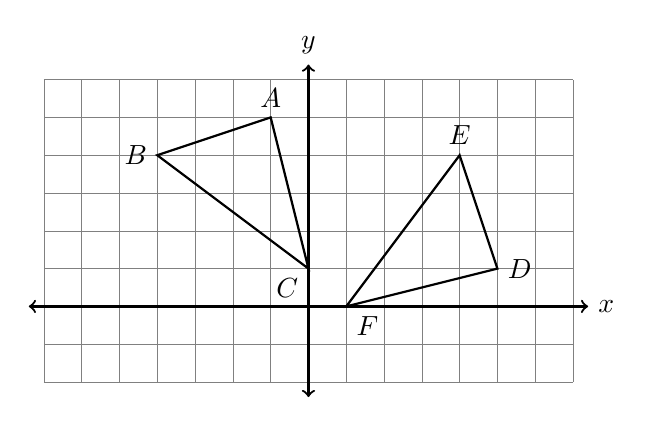
\begin{tikzpicture}[scale=.48]
        \draw [help lines] (-7,-2) grid (7,6);
        \draw [thick, <->] (-7.4,0) -- (7.4,0) node [right] {$x$};
        \draw [thick, <->] (0,-2.4)--(0,6.4) node [above] {$y$};  
        \draw [thick]
          (-1,5) node[above] {$A$}--
          (-4,4) node[left] {$B$}--
          (0,1) node[below left] {$C$}--cycle;
        \draw [thick]
        (5,1) node[right] {$D$}--
        (4,4) node[above] {$E$}--
        (1,0) node[below right] {$F$}--cycle;
      \end{tikzpicture}
    \end{flushright}
  
  \item First reflect the trapezoid $BECA$ across the $y$-axis, then move it down five and right two. Label the images $B'E'C'A'$ and $B''E''C''A''$.
    \begin{center}
        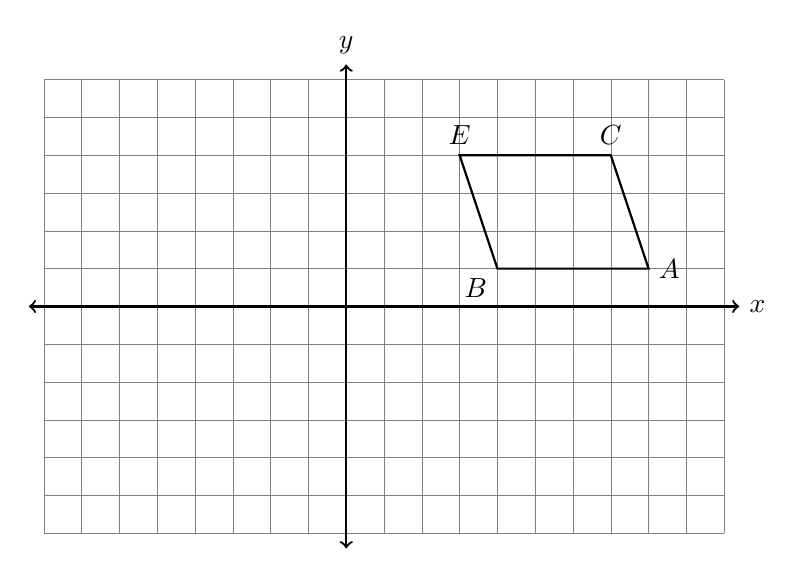
\begin{tikzpicture}[scale=.48]
        \draw [help lines] (-8,-6) grid (10,6);
        \draw [thick, <->] (-8.4,0) -- (10.4,0) node [right] {$x$};
        \draw [thick, <->] (0,-6.4)--(0,6.4) node [above] {$y$};  
        \draw [thick]
          (4,1) node[below left] {$B$}--
          (3,4) node[above] {$E$}--
          (7,4) node[above] {$C$}--
          (8,1) node[right] {$A$}--cycle;  
      \end{tikzpicture}
    \end{center}

  \item Two transformations have been applied to a triangle in the diagram below, \\$\triangle ABC \rightarrow \triangle A'B'C' \rightarrow \triangle A''B''C''$. Fully characterize each transformation.
    \begin{flushright}
        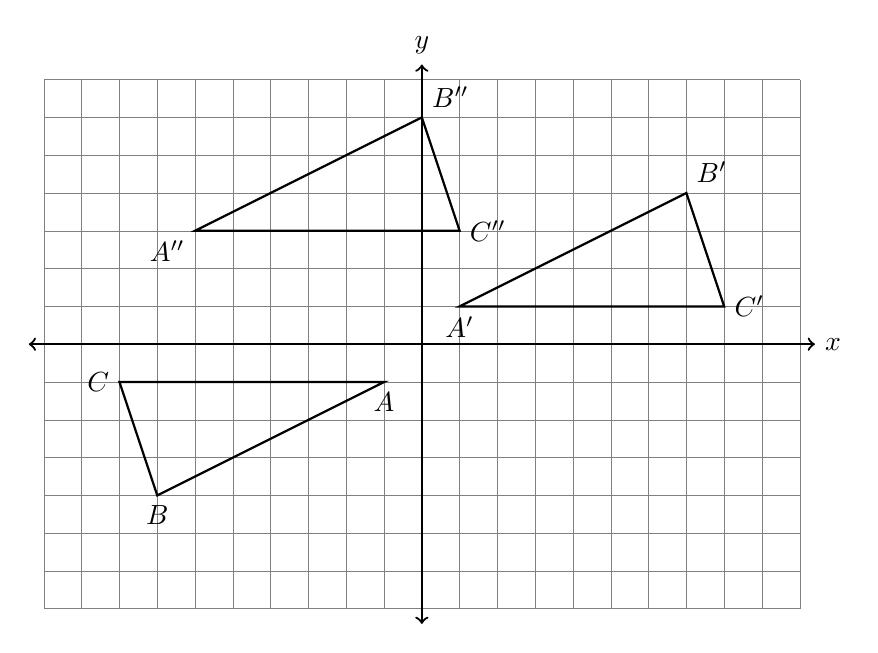
\begin{tikzpicture}[scale=.48]
        \draw [help lines] (-10,-7) grid (10,7);
        \draw [thick, <->] (-10.4,0) -- (10.4,0) node [right] {$x$};
        \draw [thick, <->] (0,-7.4)--(0,7.4) node [above] {$y$};  
        \draw [thick]
          (-6,3) node[below left] {$A''$}--
          (0,6) node[above right] {$B''$}--
          (1,3) node[right] {$C''$}--cycle;
        \draw [thick]
          (1,1) node[below] {$A'$}--
          (7,4) node[above right] {$B'$}--
          (8,1) node[right] {$C'$}--cycle;  
          \draw [thick]
          (-1,-1) node[below] {$A$}--
          (-7,-4) node[below] {$B$}--
          (-8,-1) node[left] {$C$}--cycle;
      \end{tikzpicture}
    \end{flushright} \vspace{2cm}

  \item Reflect the trapezoid $BECA$ across the $x$-axis. Label the image $B'E'C'A'$.
    \begin{center}
        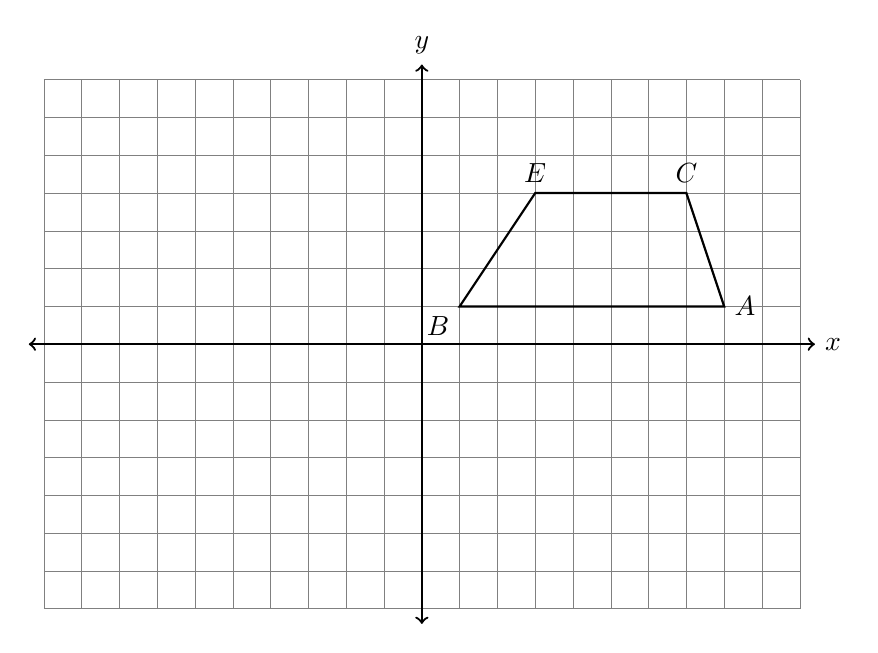
\begin{tikzpicture}[scale=.48]
        \draw [help lines] (-10,-7) grid (10,7);
        \draw [thick, <->] (-10.4,0) -- (10.4,0) node [right] {$x$};
        \draw [thick, <->] (0,-7.4)--(0,7.4) node [above] {$y$};  
        \draw [thick]
          (1,1) node[below left] {$B$}--
          (3,4) node[above] {$E$}--
          (7,4) node[above] {$C$}--
          (8,1) node[right] {$A$}--cycle;  
    \end{tikzpicture}
  \end{center}

  \item The quadrilateral $ROCK$ undergoes two transformations, shown below. Describe the sequence of transformations applied.
  \begin{flushright}
      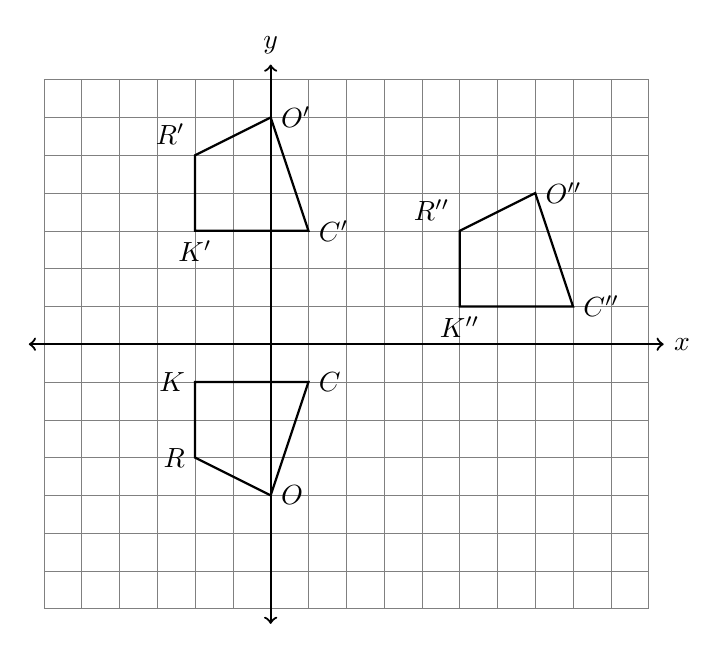
\begin{tikzpicture}[scale=.48]
      \draw [help lines] (-6,-7) grid (10,7);
      \draw [thick, <->] (-6.4,0) -- (10.4,0) node [right] {$x$};
      \draw [thick, <->] (0,-7.4)--(0,7.4) node [above] {$y$};  
      \draw [thick]
        (5,1) node[below] {$K''$}--
        (5,3) node[above left] {$R''$}--
        (7,4) node[right] {$O''$}--
        (8,1) node[right] {$C''$}--cycle;
      \draw [thick]
        (-2,3) node[below] {$K'$}--
        (-2,5) node[above left] {$R'$}--
        (0,6) node[right] {$O'$}--
        (1,3) node[right] {$C'$}--cycle;  
      \draw [thick]
      (-2,-1) node[left] {$K$}--
      (-2,-3) node[left] {$R$}--
      (0,-4) node[right] {$O$}--
      (1,-1) node[right] {$C$}--cycle;
    \end{tikzpicture}
  \end{flushright}

  \item Draw the line of reflection used to map $\triangle ABC$ onto $\triangle A'B'C'$.
  \begin{center}
      \begin{tikzpicture}%[scale=.48]
      %\draw [help lines] (-7,-2) grid (7,6);
      %\draw [thick, <->] (-7.4,0) -- (7.4,0) node [right] {$x$};
      %\draw [thick, <->] (0,-2.4)--(0,6.4) node [above] {$y$};  
      \draw [thick]
        (1,5) node[above] {$A$}--
        (3,4) node[above ] {$B$}--
        (-1,2) node[below left] {$C$}--cycle;
      \draw [thick]
      (5,1) node[right] {$A'$}--
      (4,3) node[above right] {$B'$}--
      (2,-1) node[below right] {$C'$}--cycle;
    \end{tikzpicture}
  \end{center}

  \item Draw the line of reflection for the diagram below. \\
    \begin{tikzpicture}[scale=.48]
      %\draw [help lines] (-10,-7) grid (10,7);
      \draw [thick, <->] (-4.4,0) -- (8.4,0) node [right] {$x$};
      \draw [thick, <->] (0,-2.4)--(0,7.4) node [above] {$y$};  
      \draw [thick](5,1)--(7,2)--(8,5)--(6,5)--cycle;  
      \draw [thick](-1,1)--(-3,2)--(-4,5)--(-2,5)--cycle;
    \end{tikzpicture} \hspace{1.7cm}
    
  \item Draw the line of reflection for the diagram below. \\
    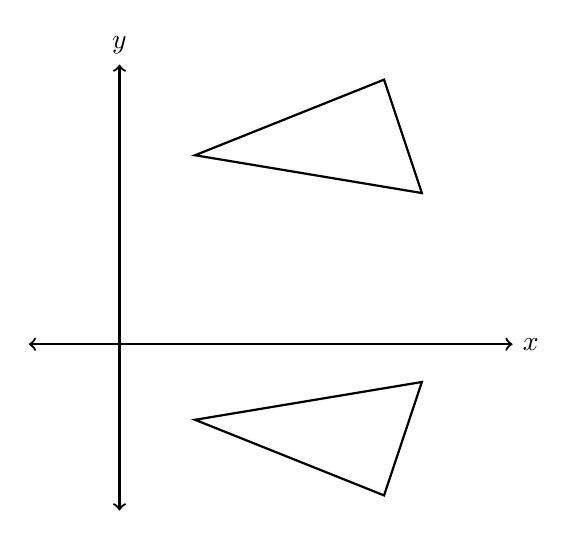
\begin{tikzpicture}[scale=.48]
      %\draw [help lines] (-10,-7) grid (10,7);
      \draw [thick, <->] (-2.4,0) -- (10.4,0) node [right] {$x$};
      \draw [thick, <->] (0,-4.4)--(0,7.4) node [above] {$y$};  
      \draw [thick](2,5)--(7,7)--(8,4)--cycle;  
      \draw [thick](2,-2)--(7,-4)--(8,-1)--cycle;
    \end{tikzpicture}

  \item Determine and state the sequence of transfromations applied to map $BECA$ to $B'E'C'A'$ and then to $B''E''C''A''$.
  \begin{center}
      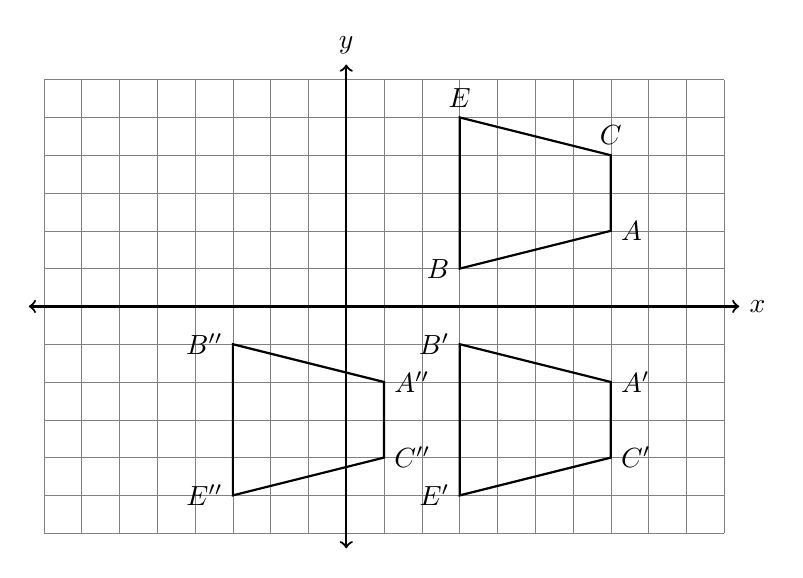
\begin{tikzpicture}[scale=.48]
      \draw [help lines] (-8,-6) grid (10,6);
      \draw [thick, <->] (-8.4,0) -- (10.4,0) node [right] {$x$};
      \draw [thick, <->] (0,-6.4)--(0,6.4) node [above] {$y$};  
      \draw [thick]
        (3,1) node[left] {$B$}--
        (3,5) node[above] {$E$}--
        (7,4) node[above] {$C$}--
        (7,2) node[right] {$A$}--cycle;
      \draw [thick]
        (3,-1) node[left] {$B'$}--
        (3,-5) node[left] {$E'$}--
        (7,-4) node[right] {$C'$}--
        (7,-2) node[right] {$A'$}--cycle; 
      \draw [thick]
        (-3,-1) node[left] {$B''$}--
        (-3,-5) node[left] {$E''$}--
        (1,-4) node[right] {$C''$}--
        (1,-2) node[right] {$A''$}--cycle; 
    \end{tikzpicture}
  \end{center}

  \item Find the image of $A(3,2)$ after a translation four to the right and down two. \vspace{1cm}
  \item Apply the translation $(x,y) \rightarrow (x-5,y+1)$ to the point $B(-2,-1)$. \vspace{1cm}
  \item State the translation that would map $C(6,3)$ onto $C'(5,13)$.

  \item Determine and state the transformation mapping $\triangle NOP$ onto $\triangle QRP$. 
    \begin{flushright}
        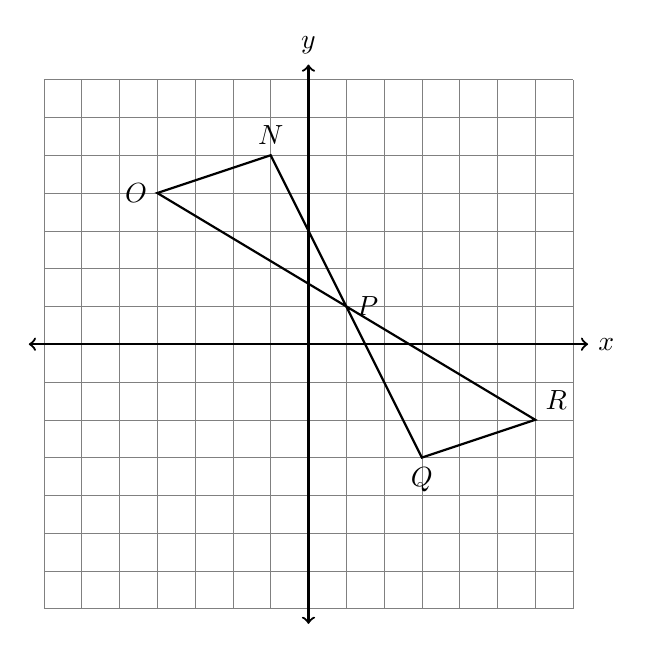
\begin{tikzpicture}[scale=.48]
        \draw [help lines] (-7,-7) grid (7,7);
        \draw [thick, <->] (-7.4,0) -- (7.4,0) node [right] {$x$};
        \draw [thick, <->] (0,-7.4)--(0,7.4) node [above] {$y$};  
        \draw [thick]
          (-1,5) node[above] {$N$}--
          (-4,4) node[left] {$O$}--
          (1,1) --cycle;
        \draw [thick]
        (3,-3) node[below] {$Q$}--
        (6,-2) node[above right] {$R$}--
        (1,1) node[right] {$P$}--cycle;
      \end{tikzpicture}
    \end{flushright}

  \item Apply the translation $(x,y) \rightarrow (x-2,y+4)$ to the point $A(2,-1)$. 
    \begin{center}
      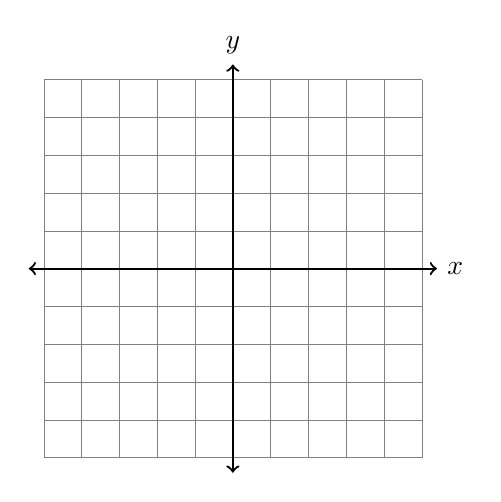
\begin{tikzpicture}[scale=.48]
      \draw [help lines] (-5,-5) grid (5,5);
      \draw [thick, <->] (-5.4,0) -- (5.4,0) node [right] {$x$};
      \draw [thick, <->] (0,-5.4)--(0,5.4) node [above] {$y$};   
    \end{tikzpicture}
  \end{center}
  
  \item What is the image of $B(2,4)$ under a reflection across the $x$-axis?
    \begin{center}
      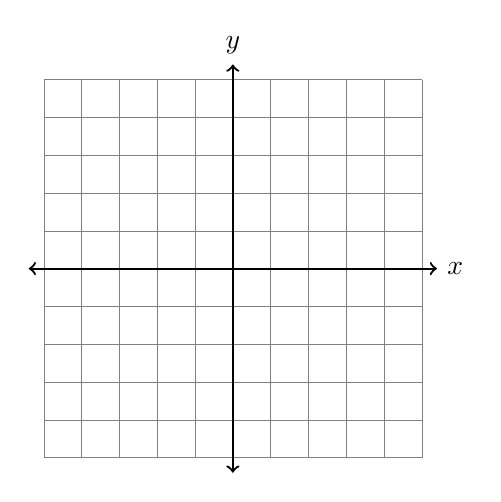
\begin{tikzpicture}[scale=.48]
      \draw [help lines] (-5,-5) grid (5,5);
      \draw [thick, <->] (-5.4,0) -- (5.4,0) node [right] {$x$};
      \draw [thick, <->] (0,-5.4)--(0,5.4) node [above] {$y$};   
    \end{tikzpicture}
  \end{center}

  \item State the translation that would map $C(-3,1)$ onto $C'(4,0)$.
    \begin{center}
      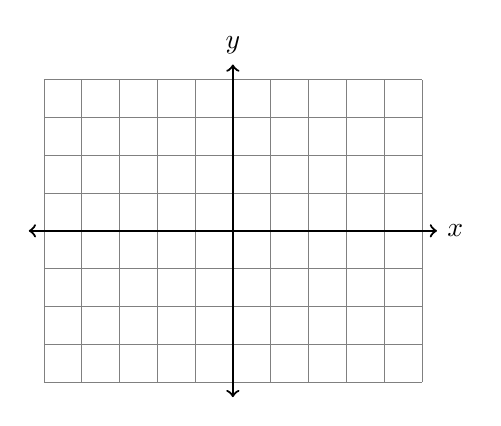
\begin{tikzpicture}[scale=.48]
      \draw [help lines] (-5,-4) grid (5,4);
      \draw [thick, <->] (-5.4,0) -- (5.4,0) node [right] {$x$};
      \draw [thick, <->] (0,-4.4)--(0,4.4) node [above] {$y$};   
    \end{tikzpicture}
  \end{center}

  \newpage
    \item Given $D(1,9) \rightarrow D'(4,3)$. Find the image of $E(6,-2)$ with the translation.
    \begin{center}
      \begin{tikzpicture}[scale=.48]
      %\draw [help lines] (-5,-5) grid (5,5);
      \draw [thick, <->] (-5.4,0) -- (5.4,0) node [right] {$x$};
      \draw [thick, <->] (0,-5.4)--(0,5.4) node [above] {$y$};   
    \end{tikzpicture}
  \end{center}
  
    \item The image of triangle $ABC$ after a translation is $\triangle A'B'C'$. Is the area of the triangle greater, smaller, or the same after the translation? Justify your answer. \vspace{3cm}
  
\end{enumerate}
\end{document}

